\documentclass[pdftex,cyrillic,14pt,a4page,twoside]{extreport}
\usepackage[bulgarian]{babel}

\usepackage[margin=2cm]{geometry}% http://ctan.org/pkg/geometry
\usepackage[pdftex]{graphicx}
\graphicspath{ {./figures/} }

\usepackage{./titlesec/titlesec}

% Counter too wide line spacing added by twoside
% https://tex.stackexchange.com/questions/62572/twoside-introduces-incorrect-linespacing-at-end-of-section
\raggedbottom
  
\titleformat{\chapter}%
  {\normalfont\bfseries\Huge}{\thechapter.}{10pt}{}

\usepackage{afterpage}
\newcommand\blankpage{%
    \null
    \thispagestyle{empty}%
    \newpage}


\begin{document}
\begin{titlepage}
	\begin{center}
	
\includegraphics[scale=1.2]{./NBU_logo.jpg}\\[0.3cm]
    \textbf{\Large НОВ БЪЛГАРСКИ УНИВЕРСИТЕТ\\[0.4cm]}
    \textbf{\Large Департамент Информатика\\[0.4cm]}
    \textbf{\Large Бакалавърка програма Информатика\\[3cm]}
   
		\textbf{\LARGE Автоматизиран биоинформатичен анализ на генетични варианти, потенциално свързани със стареенето\\[2cm]}
		\begin{Large}
		Дипломна работа на\\[0.2cm]
		Михаил М. Здравков\\[3cm]
		\end{Large}
		\begin{minipage}{0.48\textwidth}
			\begin{flushleft} \large
				\emph{Научни ръководители:} \\
				доц. д-р Милена Георгиева \\
				Момчил Топалов
			\end{flushleft}
		\end{minipage}
			\begin{minipage}{0.48\textwidth}
			\begin{flushright} \large
				\emph{Ръководител катедра:} \\
				гл. ас. д-р Методи Трайков\\
				\clearpage
			\end{flushright}
		\end{minipage}

		\vfill

		% Bottom of the page
		{\large София 2022}

	\end{center}
\end{titlepage}


\afterpage{\blankpage}

\newgeometry{
	inner=30mm,
    outer=20mm,
    top=20mm,
    bottom=20mm}

\tableofcontents
\pagebreak
\afterpage{\blankpage}



\chapter{Увод}
\paragraph{}

Стареенето е естествен процес, който има огромно значение както за отделния индивид, така и за обществото като цяло. С напредването на възрастта, рискът от разнообразни заболявания като рак, болест на Алцхаймер, диабет, сърдечно-съдови заболявания и др. нараства значително. Смята се, че около две-трети от смъртните случаи при хора се дължат на заболявания, свързани с възрастта. Същевременно, с глобалното нарастване на средната продължителност на живота, проблемите на стареенето засягат все повече хора и имат все по-голямо обществено значение. От социална гледна точка, стареенето оказва значителен икономически и демографски ефект.

\paragraph{}
Установено е, че процесът на стареене се влияе както от генетични, така и от епигенетични фактори. Въпреки това, този процес все още не е достатъчно добре разбран от науката, поради което е трудно да се създадат ефективни методи за терапия и справяне с негативните му ефекти.

\paragraph{}
Основен подход при изследването на генетичната основа на стареенето е анализът на генетични варианти. При такива изследвания е необходима обработката на големи обеми от данни, което налага нуждата от използване на специализиран биоинформатичен софтуер. Налични са множество различни инструменти, покриващи различни аспекти от обработката на файлове с генетични варианти - анотация, филтриране, анализ и тн. Повечето от тях, обаче, изискват значителни технически познания, което ги прави трудни за използване от специалисти в други области, като биология и генетика.

\paragraph{}
Целта на настоящата дипломна работа е създаването на интегрирана софтуерна система за биоинформатични изследвания на генетични варианти и предсказване на тяхната потенциална асоциация с процеса на стареене. Надяваме се, чрез създаване на по-достъпен инструмент, да допринесем за бъдещи изследвания на процеса на стареене и за търсенето на ефективни терапии против негативните му ефекти.
            
\chapter{Литературен обзор}
\section{Значение на стареенето}
\subsection{Дефиниция}
\paragraph{}
Въпреки, че концепцията за стареене е универсално разбираема, формалната ѝ дефиниция не е тривиална и множество автори дават твърде различни определения за този термин. Аркинг (2006, стр. 11) прави преглед на наличната литература и, в резултат, предлага следната дефиниция\cite{arking2006biology}:

\paragraph{}
\textit{„Стареенето е независима от времето поредица от кумулативни, прогресивни, свойствени и вредящи структурни и функционални промени, които обикновено започват да се изразяват при репродуктивната зрялост и приключват със смъртта.“}

\paragraph{}
Макар времето да няма каузална връзка с ефектите на стареенето, то корелацията помежду им е причина обикновено да се говори за ефектите на стареенето като за нещо, настъпващо с напредването на възрастта.

\subsection{Физиологични ефекти}
Стареенето оказва изключително голям ефект върху човешкото тяло. То обикновено включва широк спектър от различни физиологични промени, повечето от които влошават жизнеността и качеството на живот на индивида. Примери за това са понижена фертилност при жените\cite{kamath2010}, загуба на телесна маса\cite{spencer1996}, влошен слух\cite{feder2015}, повишен риск от хронични заболявания\cite{larson2013}\cite{prasad2012}, хронична болка\cite{geriatrics2002} и др.


\subsection{Демографски и икономически ефекти}
През последния един век очакваната продължителност на живота в целия свят драстично се е повишила\cite{zijdeman2016} (виж фиг. \ref{fig:life_expectancy}). Освен безспорните ползи, това води и до редица проблеми. Удължаването на продължителността на живота, в комбинация с наблюдавания спад на раждаемостта, се очаква да доведе до застаряване на населението\cite{lutz2008}. Световната Здравна Организация (СЗО) предупреждава, че се очаква между 2015 и 2050 броят на хората над 60-годишна възраст да се повиши от 12\% от населението до 22\%\cite{who_report_ageing2015}. Същевременно, по данни на СЗО, увеличаването на продължителността на живота (с 6 години за периода между 2000 и 2019) изпреварва увеличаването в продължителността на здравословния живот (с 5.4 години за същия период)\cite{who_health2020}. \\
\begin{figure}[h]
  \centering
  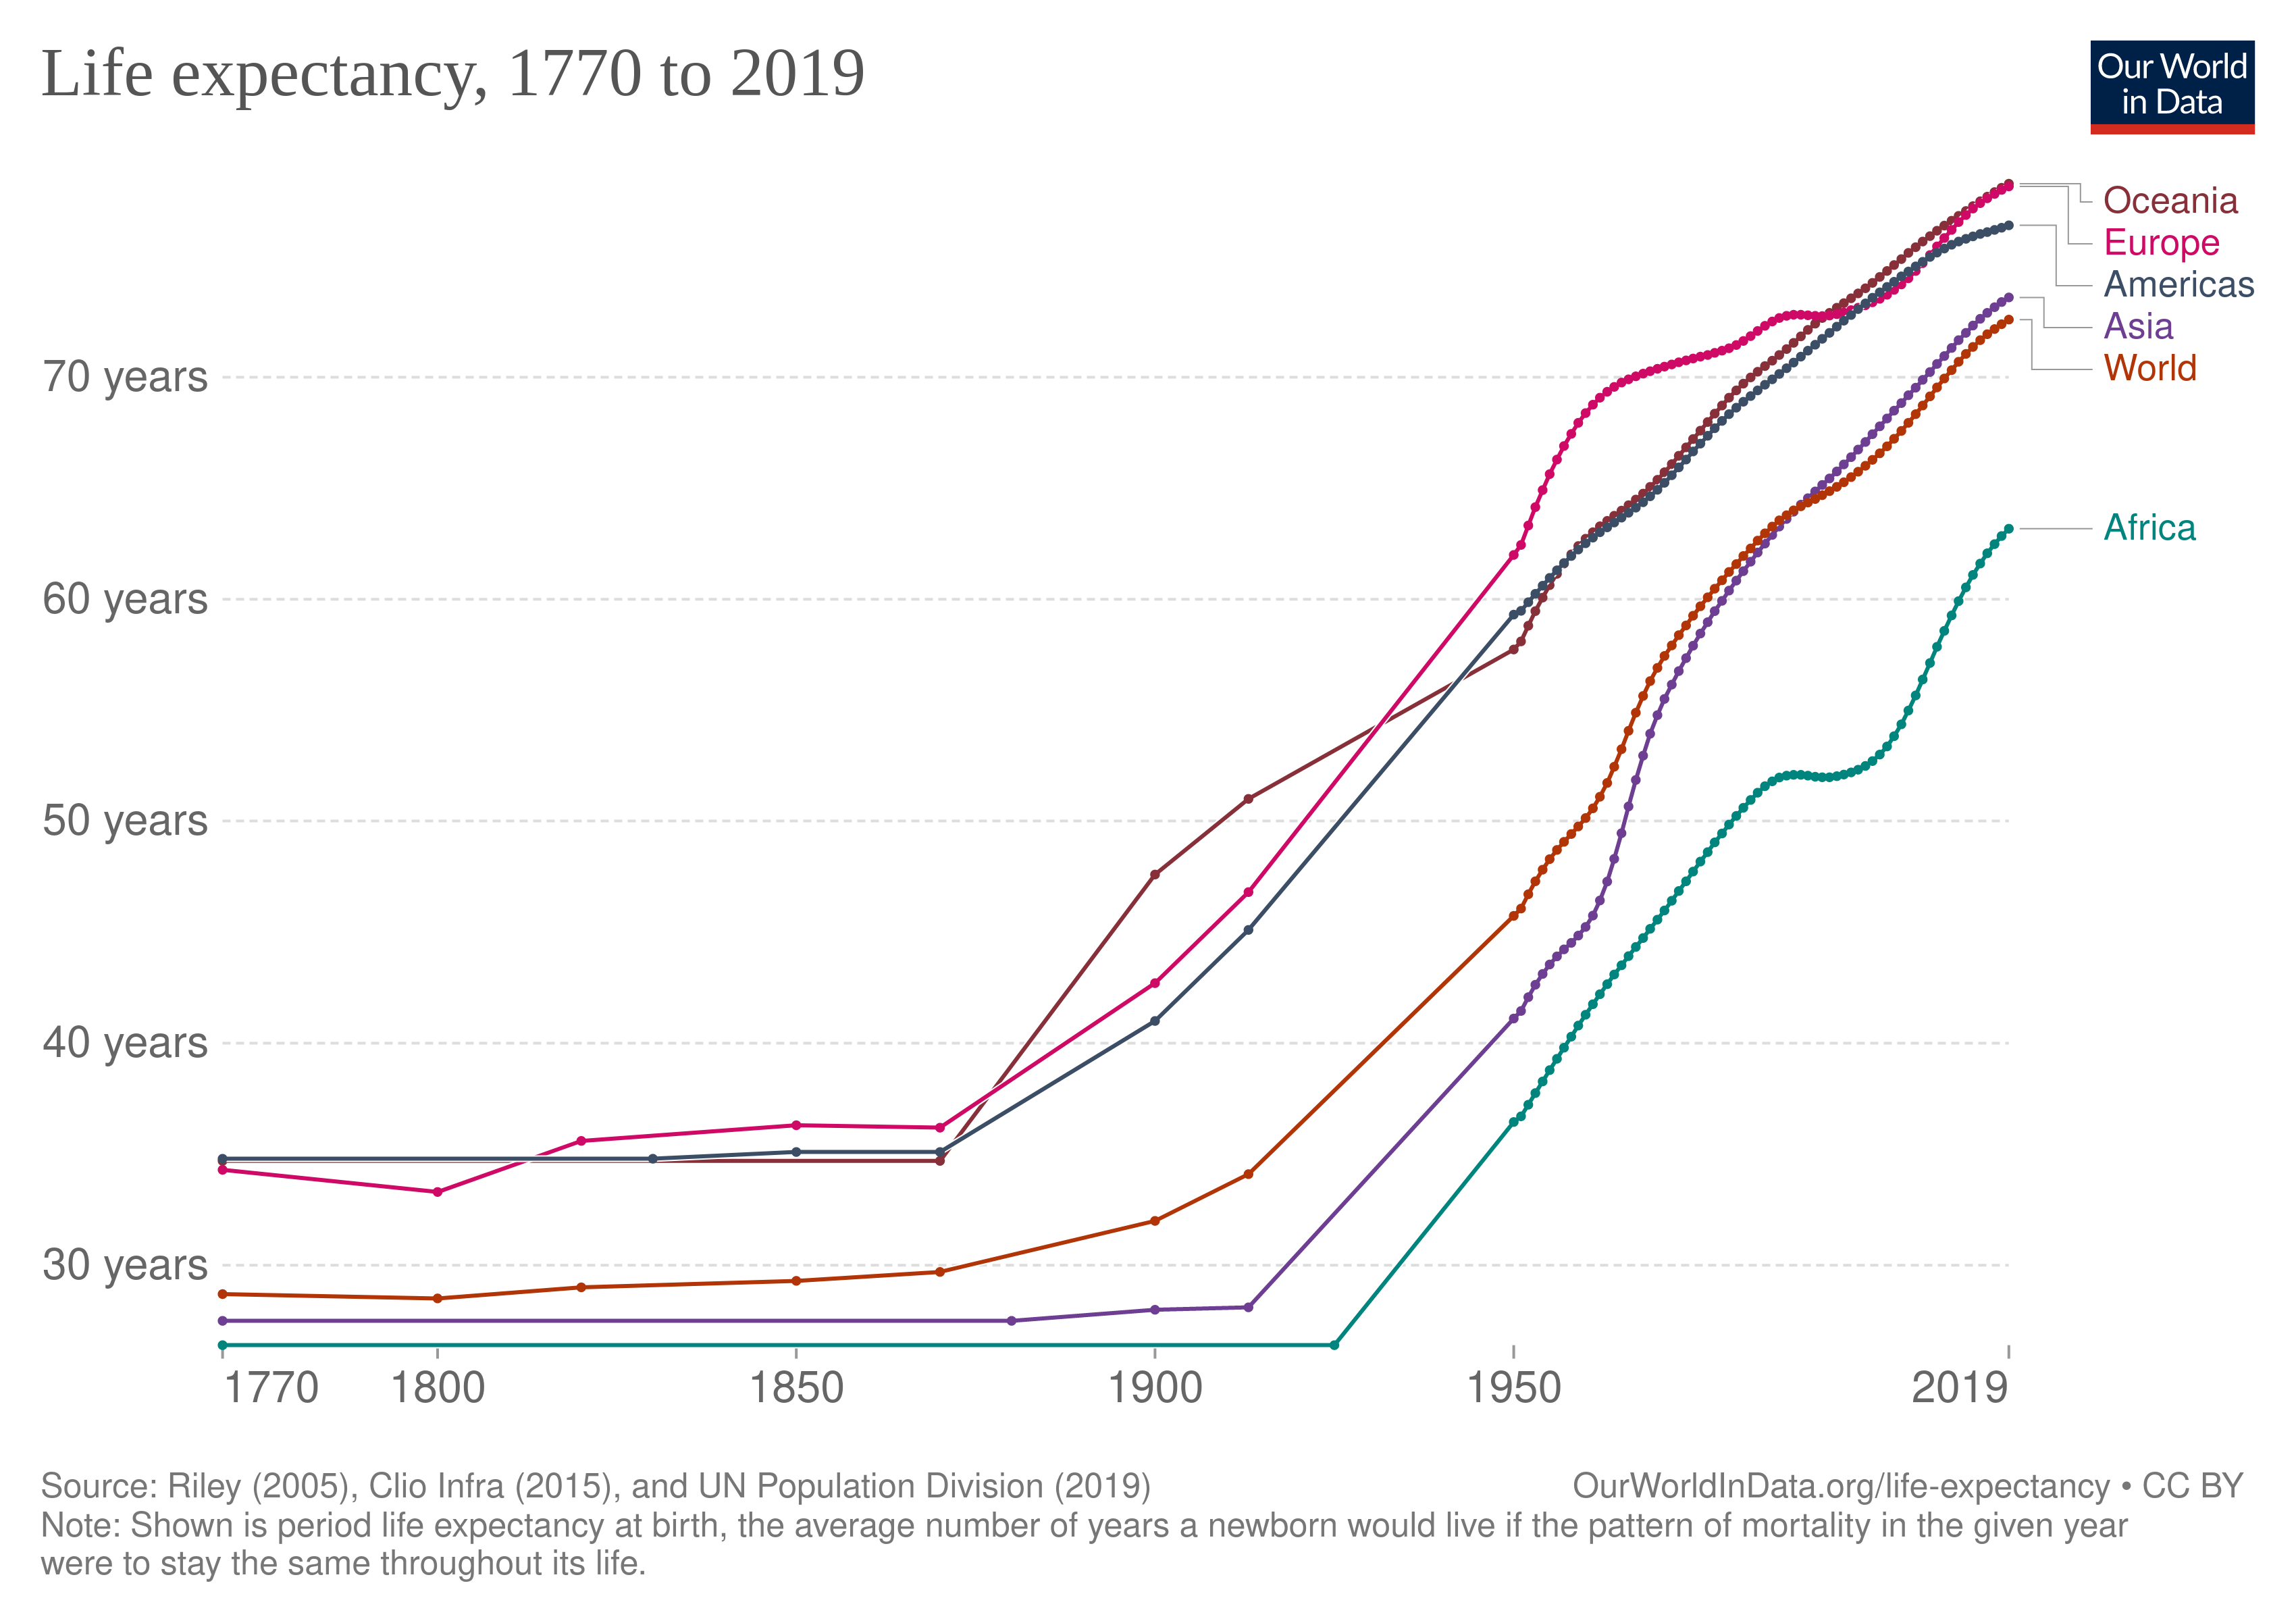
\includegraphics[width=12cm]{figures/life-expectancy}
  \caption {Очаквана продължителност на живота за различни региони}
  \label{fig:life_expectancy}
\end{figure}

\paragraph{}
Застаряването на населението би оказало неблагоприятен ефект и върху икономиката на държавите. Първо, заради увеличаването на дяла на хора, които не участват в работната сила. Второ, поради това, че здравните системи ще бъдат допълнително натоварени с по-голям брой хора в напреднала възраст, за които рисковете от хронични заболявания са значително по-големи.


\section{Биологичес}

\chapter*{Използвани външни\\ библиотеки и софтуер}
\addcontentsline{toc}{chapter}{Използвани външни библиотеки и софтуер}

%\chapter*{Използвана литература}
%\addcontentsline{toc}{chapter}{Използвана литература}

\bibliographystyle{plain}
\bibliography{refs}
\addcontentsline{toc}{chapter}{Библиография}

\end{document}